\documentclass{report}
\usepackage[english]{babel}
\usepackage{microtype}
\usepackage{amsmath,amssymb}
\usepackage{amsthm}
\usepackage[round, authoryear]{natbib}
\usepackage[all]{xy}
\usepackage{graphicx}
\usepackage{framed}
\usepackage{enumerate}
\usepackage{qtree}
\usepackage{mdframed}
\usepackage{tikz-dependency}
\usepackage{float}
\bibliographystyle{plainnat}
\author{}
\title{}

%Define theorem style for definition and metric
\theoremstyle{definition}
\newtheorem{metric}{Metric}
\newtheorem{notion}{Notion}
\theoremstyle{plain}
\newtheorem{definition}{Definition}
\def\citepos#1{\citeauthor{#1}'s (\citeyear{#1})}

%Define new float environment for tables that is boxed
\floatstyle{boxed}
\newfloat{tab}{tbp}{lop}
\floatname{tab}{Table}


\begin{document}
\maketitle
\tableofcontents



%%%%%%%%%%%%%%%%%%%%%%%%%%%%%%%%%%%%%%%%%%%%%%%%%%%%%%%%%%%%%%%%%%%%%%%%%%%%%%%
%%%%%%%%%%%%%%%%%%%%%%%%%%%%%%%%%%%%%%%%%%%%%%%%%%%%%%%%%%%%%%%%%%%%%%%%%%%%%%%

\chapter{Introduction}

%%%%%%%%%%%%%%%%%%%%%%%%%%%%%%%%%%%%%%%%%%%%%%%%%%%%%%%%%%%%%%%%%%%%%%%%%%%%%%%
%%%%%%%%%%%%%%%%%%%%%%%%%%%%%%%%%%%%%%%%%%%%%%%%%%%%%%%%%%%%%%%%%%%%%%%%%%%%%%%


% Introduction to machine translation, quote Warren Weaver

\begin{quote}
\textit{When I look at an article in Russian, I say: `This is really written in English, but it has been coded in some strange symbols. I will now proceed to decode.}
\end{quote}

Evidently, automatic translation is not as easily solved as Weaver thought at the time. Over 60 years later, the state-of-the-art systems are still not able to produce translations of an arbitrary text with a quality compared to that of a translation of a human translator.

%How big did machine translation get

and many different methods have been investigated. This work focuses on one such method: compositional translation.


%Describe compositional translation
%Explain why compositional translation is attractive from a theoretical point of view.

In many fields in which translations occur (computer science, logic, philosophy), computational translation is a very common method. The semantics of an expression in a certain logic, for instance, can be unambiguously determined by considering the terms and the methods used to combine them. Translating such an expression into another logical language can be effectively carried out by translating these terms and methods into the terms and methods particular for the second logic.

%Explain why for language it is not so straight forward that we can do this: words have multiple meanings, sentences are vague and ambiguous, building blocks unclear
%Explain that we also do not a-priori dispose over grammars and mappings, as we did not design natural languages as artificial languages, nor is it clear of such mappings even exist.


% although not every grammar is suitable for compositional meaning assignment, the class of languages that can be analyzed is not restricted, nor are the meanings that can be assigned: any recursively enumerable language can be generated by a compositional grammar, and any semantics can be dealt with in a compositional way. 
%Is this helpful? Is NL recursively enumerable? What about ambiguity

However, none of this teaches us if compositional translation is a reasonable strategy for translating natural language. Intuitively, it seems reasonable that 'who-did-what-to-whom-relations' are universal for languages, but exploiting this fact in translation has proven to be a non-trivial task. The present work does not aim to develop a model for compositional translation of language, but rather attempts to empirically analyse if it is realistic to aim for one.\\
%Explain how this question becomes practical
Although this question is of theoretical nature, blabla explain that we have to deal with data such that it merely transforms to the question: can we find compositionality in the corpora we are training on, that an be of use in translation models. We will therefore also pay some attention to the use of the results, and make suggestions for future work.


\section*{Thesis Outline}

%Rewrite this when the rest is written
As mentioned before, the primary goal of this thesis is to investigate whether predicate-argument relations are preserved during translation. To do so, a tree will be searched that respects both the alignment (completely) and as much of the predicate-argument relations present in the source sentence as possible. The resulting tree will be scored according to how many of the predicate argument relations were allowed by the alignment, thus yielding a compositionality measure for the sentence.\\
The following chapter will give some theoretical background: it will explain the notion of alignment-respecting trees (anders) and provide some information on the grammar formalism used to extract predicate-argument relations.\\
Chapter give more information on the implementation of the research, while the actual experiments and their results will be presented in chapter 
%We probably also need a section about compositionality (lets see how that is gonna fit in)
%Describe the rest





%%%%%%%%%%%%%%%%%%%%%%%%%%%%%%%%%%%%%%%%%%%%%%%%%%%%%%%%%%%%%%%%%%%%%%%%%%%%%%%%%%%%%%%%%%%%%%%%%%%%%%%%%%%%%%%%%%%%%%%%%%%%%%%%%%%%%%%%%%%%%%%%%%%%%%
%%%%%%%%%%%%%%%%%%%%%%%%%%%%%%%%%%%%%%%%%%%%%%%%%%%%%%%%%%%%%%%%%%%%%%%%%%%%%%%%%%%%%%%%%%%%%%%%%%%%%%%%%%%%%%%%%%%%%%%%%%%%%%%%%%%%%%%%%%%%%%%%%%%%%%
%BACKGROUND ON MT AND TRANSFER MODELS

\chapter{Transfer Models in Machine Translation}



Machine translation is a very complex problem, to which many approaches have been tried. In this thesis, we focus on one such approach: the transfer method.   After a short introduction to the beginning of machine translation (MT), the focus will thus mainly lay on models that use this method. It does not claim to give a complete overview of these; MT is an enormous field in which many models have been developed, most of which are hybrid in the sense that they borrow from different approaches to complete different parts of translation. For more complete overviews of MT and SMT, the reader is referred to \cite{hutchins1992introduction} (MT), \cite{somers1999review} (EBMT) and \cite{koehn2008statistical} (SMT).


\section{Early Transfer Models}
%Reference to early transfer models?
Machine translation was, rising as a field of research almost immediately after the emergence of the first computers, one of the very first problems to be tackled by computers. The very first approaches to solve the problem, also called the first generation approaches, were more or less direct: sentences were treated as structureless sequences of words that can be directly mapped to words in another language. Using this approach, relations between words or other structural aspects of the sentence are thus not considered. Clearly, such a strategy is only reasonable if source and target languages are structured almost identical: a translation whose structure deviates from the structure of the original sentence will never be found. Unfortunately for MT researchers, natural languages are not ordered in this fashion, and the direct approach of the first generation models was not very successful. First generation models often lead to translations that were incomprehensible, not fluent and often not even meaning preserving.\\
The failure of the first generation models lead to a second generations of models, using indirect methods, that laid the groundwork for the models considered in this paper. The main idea of the second generation systems was to analyse the source sentence into an intermediate representation that was supposed to somehow convey the semantic structure (or `meaning') of the sentence, and map this representation to an intermediate representation in the target language. From this intermediate representation, the translation of the sentence in the target language could be derived. The process of mapping representations in one language to representations in another is called transfer.\\
An extreme case of the transfer method is the one in which the intermediate representation is a universal one. Such a representation, called interlingua, can be seen as a description of the meaning of the sentence independent of any natural language. The transfer part is therefore reduced to the identity mapping, and translation consists of translating the sentence to an independent meaning representation and deriving the target sentence from this representation. This is attractive from a theoretical point of view, as it addresses the problem of translation on a fundamental level, but is very hard, especially when the meaning space is unrestricted. Some researchers have succeeded in writing rather successful translation models for very small domains (give examples!!), but nowadays, finding a formal semantics that can capture all of human language is an independent research field, in which a satisfiable interlingua has not yet been found.

\begin{figure}[!ht]
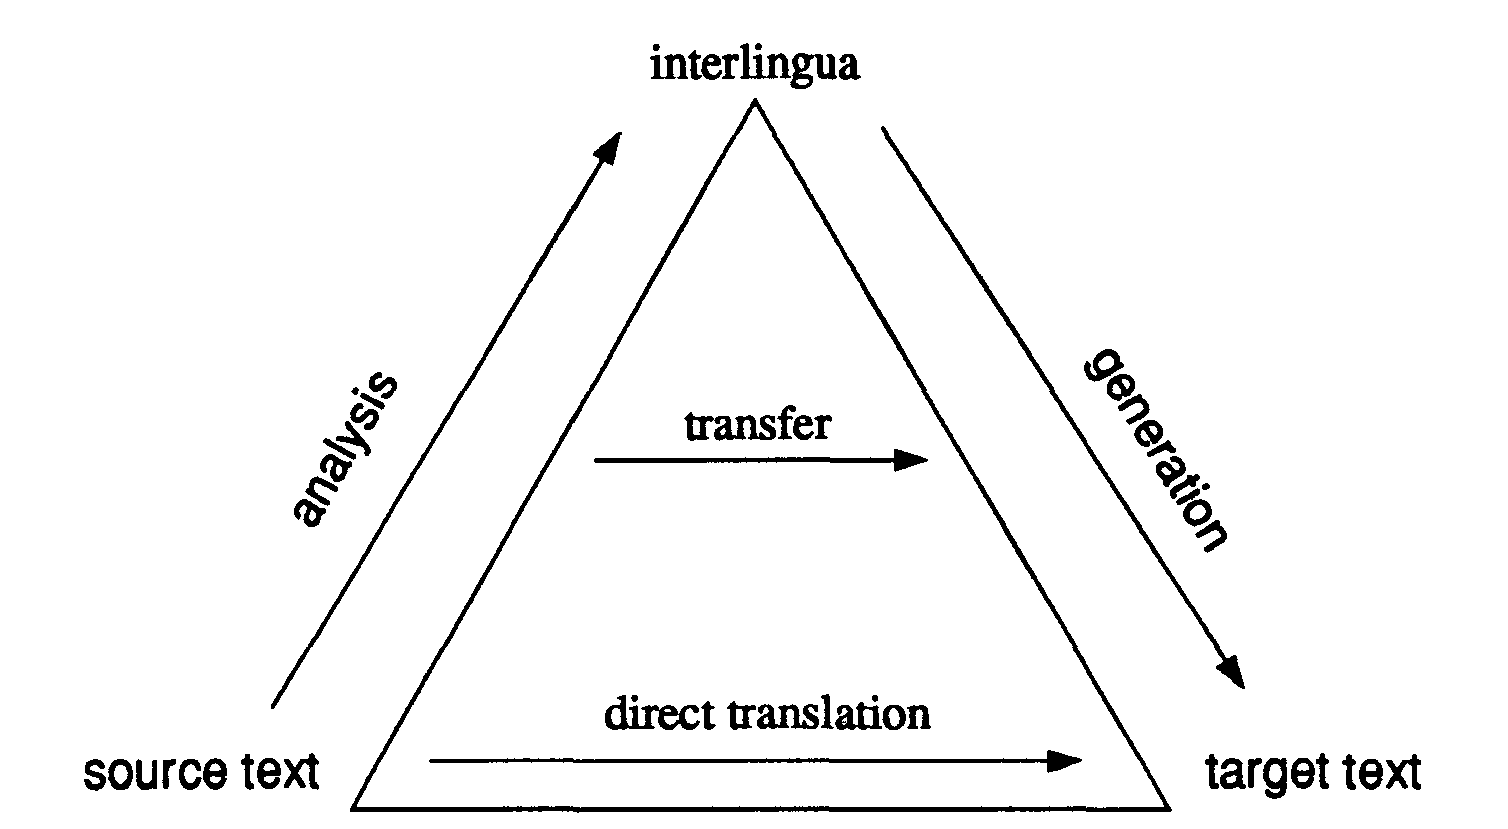
\includegraphics[scale=0.2]{translation_triangle.png}
\caption{Vauquois pyramid?}\label{fig:triangle}
\end{figure}

The three translation methods described can be pictured in a pyramid, showing how they are related (Figure \ref{fig:triangle}). This pyramid also shows that, although direct translation and interlingua are two inflexible extremes, the tranfer method can be employed in different ways, varying the distance from source and target text to intermediate representation (analysis and generation, respectively), and with this the distance between the intermediate representations.

\section{Early Statistical Models}

Driven by the thought that language it too rich to formalize, a new line of research came of the ground, that was not primarily based on linguistic knowledge, but on large pairs of text that were translations of each other (parallel corpora). In the beginning, the corpus based systems seemed to be rival to the existing linguistically oriented paradigm, but soon people concluded that the two approaches were not actually conflicting, and nowadays most models combine the two of them.\\
Corpus based models can be roughly divided into two main categories.\footnote{Although this division has some theoretical ground, it is mainly suggested to be able to distinguish work that is interesting for this paper and work that is not.} Models of the first category are directly based on analogy. When translating a sentence, they try to find examples in the corpus similar to (fragments of) the sentence and generate a translation by recombining them. This part of machine translation is often called Exemplar Based Machine Translation. Early EBMT models will not be further discussed (a detailed discussion can be found in \cite{somers1999review}). The early MT researchers had the misfortune that computational standards were not as they are today and their models often only treat small sub languages, are computationally not executable and certainly not scalable. Many of the idea's investigated came back in later papers about MT (e.g. consider \citepos{furuse1992example} hierarchical phrases), although it is unclear if they were inspired by earlier papers or just reinvented.\\
The second category of corpus-based models is more interesting to the current work. In models of this category, appositely called statistical machine translation models, parallel corpora are not used to match and recombine, but to statistically decide on the parameters of another model. Even though the first statistical models seemingly took a step back, moving towards the direct translation approach again, and considered no linguistic information whatsoever, they were (at least result wise) an enormous improvement to any model existing at the time. As these systems were primarily word-based, they do not fall into the category of models discussed in this thesis. However, the models we will discuss are founded on the notions and concepts introduced with these first word-based models, so we will devote a section to them (and their phrase-based extension) nevertheless, before getting back to transfer-models.

\subsection{Statistical Word-based Models}

The first working statistical MT model, inspired by  Weavers idea to use information theory to reach automatic translation \citep{weaver1955translation}, was presented by \cite{brown1990statistical}. This paper was based on earlier work of the same research group \citep{brown1988statistical}, and was further worked out in a later paper \citep{brown1993mathematics}. Their models, now known as `IBM model 1-5' follow the noisy channel approach, modelling the probability $P(t|s)$ that $t$ is the translation of $s$.\footnote{In the literature, this probability is often expressed as $P(e|f)$, as the first IBM models were focussed on translation from French to English. However, this can be quite confusing for the reader, and in this paper we will stick to the more general $t$ for target and $s$ for source.} This probability is then expressed using Bayes' theorem resulting in the following expression (by the authors called The Fundamental Equation of Machine Translation) for the desired translation $\hat{t}$:

\[
\hat{t} = \operatorname*{arg\,max}_t P(t)P(s|t)
\]

The translation task is now split in two: modelling the translation probability $P(s|t)$, and modelling the language probability $P(t)$. The model for $P(t)$, that is standard an n-gram model, is meant to account for fluency of the target output. The generative model is standard in information theory, the crux of the model resides in how $P(s|t)$ is modelled. In the IBM models, this distribution is modelled by marginalizing over all possible ways in which the words in $t$ could have been generated by the words in $s$, thus $P(s|t) = \sum_a P(s,a|t)$, in which $a$ describes the mapping from target to source words. The 5 IBM models differ in the complexity of the approximation of the conditional probability $P(s,a|t)$, ranging from a very simple distribution in which $a$ is not considered at all (in which case the probability is independent of word-order) to rather complex ones in which $a$ is dependent on several parameters (details can be found in \cite{brown1993mathematics}).\\
All IBM models require a lexical translation probability (i.e. a dictionary like function that specifies the probability of word $w_s$ translating into $w_t$. These probabilities are not directly observable from the parallel corpus (as the corpus is sentence aligned, and not word aligned) and are learned from the data applying the expectation maximization algorithm, that is proved to converge to a global optimum. The IBM models are nowadays not in use any more, outperformed by newer more sophisticated models, their techniques for generating word-alignments are still often used to analyse translation data, or to generate training data for newer models.


\subsection{Statistical Phrase-based Models}

The statistical IBM models led to a huge improvement in translation quality, but they still had the same drawbacks as the first generation of direct translation models: no structure or local context was considered and a large amount of natural language phenomena could therefore not be accounted for. A major leap forward was taken with the introduction of (non linguistic) phrases as basic units in translation models (\cite{wang1998grammar,och1999improved}??). A phrase translation pair is a pair of contiguous source and target sequences such that the words in the source phrase are aligned only with words in the target phrase, and vice versa. \citep{och2004alignment}. Phrases are thus not restricted to linguistic phrases, but can be any arbitrary contiguous sequence of words. Keeping the architecture (more or less) the same, using phrases instead of words as translation units allows the model to use local context during translation. Phrases based translation models can therefore capture short contiguous idiomatic translations, as well as small insertions and deletions and local reordering. E.g. both `la casa' and `il casa' are reasonable word-for-word translations of the English phrase `the house'. `il casa' is, however, not a grammatical string in Italian. The latter observation could be easily captured by a phrase-based model, as `the car' could be translated as one unit, but would be much harder to model in a word-based model. Furthermore, a word-based model would never be able to get the correct idiomatic translation of a phrase like 'kick the bucket', while a phrase-based model would have little trouble finding this translation (provided this specific idiomatic phrase was present in the training corpus). However, such models still suffer from the fact that no structure beyond the phrase level is taken into account.\footnote{Moreover, phrase based translation knows many practical problems, that will not be further discussed here. A rather detailed discussion of the (theoretical and practical) problems with phrase-based translation can be found in \cite{quirk2006we}} Attempts to incorporate syntactic structure by linguistically motivate the selection of phrases \cite{koehn2003statistical} turned out unfruitful, and the focus of the MT-world shifted back to more structure-based models.

\section{Statistical Transfer Models}

The shift of the field to more transfer-based models did not happen overnight. Some researchers were exploring statistical rule-based models even before the first phrase-based model was presented. Over the last 15 years, \textit{very} many models exploring structure beyond the phrase-level have been presented, many of which were hybrid models combining several different strategies. In this section, the focus lies on the different strategies that can be employed to find a mapping between source and target language structures. This means that this section is by no means a complete overview of the statistical syntax-based translation models over the last 15 years. We will not discuss approaches that use the recursive properties of languages without explicitly searching for a mapping, excluding for instance approaches that use syntactic structure as features in a log-linear model (e.g. \cite{cherry2013improved,liu2010semantic}), for reordering preliminary to translation (e.g. \cite{khalilov2012statistical}), to rerank output of a standard phrase-based system (e.g. \cite{och2004smorgasbord}). Also, we will not discuss the methods used to learn a probability model over the selected rules, nor will we discuss decoding or give details on the performance of the models, as it is often hard to tear apart whether performance is due to improved mappings or other factors (as better decoding strategies, different datasets or a better probability model). Furthermore, note that the models are not presented in a chronological order, but are merely grouped according to similarity (anders).

\subsection{Synchronous Context Free Grammars}
The lion's share of the statistical transfer mappings searchers for a bijective relation between source and target structure, hereby assuming that former and latter are isomorphic. The grammars and relation between them can be formalized as a synchronous context free grammar, simultaneously generating source and target structure. Even approaches that are not explicitly concerned with SCFG's can often be interpreted as such. An SCFG is defined as a set of rules of the form:

\[
X \to \langle \gamma , \alpha , \sim \rangle
\]

In which $\gamma$ and $\alpha$ are sequences of terminals and non terminals in the source and target language, respectively, and $\sim$ is a one-to-one correspondence between $\gamma$ and $\alpha$, indicating that they are translation equivalent. SCFG's implicitly model reordering phenomena and non-contiguous phrases.

\subsubsection{Strictly Linguistic SCFG's}

%(anders)
In a purely linguistic SCFG, $\gamma$ and $\alpha$ are restricted to rules allowed by linguistic monolingual grammars for the languages. The SCFG is then found by parsing both source and target sentences with a linguistic parser and aligning the trees on the node level. Although a number of early attempts can be found \citep[see][p. 20]{wu1997stochastic}, there are no recent approaches using such a `parse-match-parse'-method on the context-free level. As monolingual grammars are not designed for translation purposes it is often impossible to statistically align every source tree node to a target tree node, because the trees are not isomorphic.\footnote{Often, it would be possible to design more compatible grammars for the languages, if the goal of translation was kept in mind. (anders) A more detailed discussion of this issue can be found in \cite{rosetta1994compositional}} Current translation models whose rules are based strictly on monolingual grammars are therefore rarely context-free. Furthermore, the `parse-match-parse' method requires appropriate and robust monolingual grammars on both source and target side, as well as high quality parsers, which clearly restricts the number of languages pairs that can be treated in such a way.

\subsubsection{Strictly Formal SCFG's}

\cite{wu1997stochastic} presents a model that attacks the weaknesses of the purely linguistic approach. His framework, the inversion transduction grammar (ITG) is at the heart of many later approaches. Also the ITG framework can be formulated as an SCFG, and thus does not differ from aforementioned linguistic approaches in this aspect. However, ITG-rules are not restricted to linguistic rules, but are motivated by the translation data. The nodes in the tree are thus not necessarily linguistic constituents, but can cover any part of the sentence, as long as a translation equivalent span can be found in the other sentence. In this context, translation equivalence is defined in terms of alignments: a source and target phrase $\alpha$ and $\beta$ are translation equivalent if words in $\alpha$ are linked only to words in $\beta$ and vice versa. For isomorphic trees, it is added that $\alpha$ and $\beta$ are contiguous sequences in source and target sentence, respectively.\\
Learning formal grammar rules is associated with computational issues. Without a restriction on labels or the rank of the rules, the number of rules that can be extracted from a sentence of length $n$ grows exponentially with $n$ and hence it is impossible to include them all in a grammar. Several solutions have been proposed to this problem. \citeauthor{wu1997stochastic} himself restricts his grammar to (left-branching) binary trees with a single non-terminal, asserting that he was unable to find any real-life examples of translations that could not be explained by such trees. \cite{chiang2005hierarchical} constructs a grammar with rules containing both non-terminals (once again only a single non-terminal label is used) and terminals. The number of such translation rules is still very large ($\mathcal{O}(n^6)$ for a 1-1 monotone sentence pair \citep{quirk2005dependency}), \citeauthor{chiang2005hierarchical} prunes his rules by, i.a., putting restrictions on the length of the terminal sequences on both sides, as well as on the rank of the rules. The framework introduced by \citeauthor{chiang2007hierarchical}, combining the strengths of rule-based and phrase-based translation models, is often called hierarchical phrase-based translation. \\
Another phrase-based hierarchical model was presented in \cite{mylonakis2010learning}. The set-up is similar to \citepos{chiang2007hierarchical}, but two extra non-terminals are added to decode whether a phrase-pair tends to take part in order switching, and the rules are restricted to binary. They show that it is possible to train a complete all-phrase binary grammar with cross validated EM. \cite{blunsom2008bayesian} use a corpus to induce non-terminal categories for phrasal translations, using a Bayesian model.

%Put \cite{alshawi2000learning}
% Put \cite{menezes2003best}??

\subsubsection{Linguistically motivated formal SCFG's}

A way of reducing the rule-space in a more guided way is to use linguistic knowledge to reduce the space of possible node spans. Although such a strategy is not possible for every language pair, as it reinstates the second problem of purely linguistic transfer models, using available syntactic or semantic knowledge can result in robust models that yet do not ignore our knowledge of language and, moreover, simplify the parsing process. Both \cite{zollmann2006syntax} and \cite{almaghout2010ccg} gained performance by augmenting grammars with syntactically motivated non-terminal labels, based on standard constituency grammars and ccg, respectively. \cite{li2013modeling} integrated more semantically oriented notations in a standard hierarchical phrase-based system.


\subsection{Beyond Context Free}

Although this is formally desirable, there is no a priori reason to assume that it is possible to find isomorphic tree pairs for sentences that are each others translation. More powerful transformation methods might be more suitable for the expressive syntactic transformations going on in translation of natural language. As the necessity of deviating from conventional syntax is smaller, models of this class tend to stay closer to traditional linguistic structures.

\subsubsection{Synchronous Tree Substitution Grammars}

The class of Synchronous Tree Substitution Grammars (STSG's) is a strict superset of the class of SCFG's, and STSG's are therefore a natural extension to them. Models working with STSG's are i.a. \cite{poutsma2000data} and \cite{galley2004s,galley2006scalable}. The core method of the former is to align chunks of parse trees of source and target sentences, and transform them into rules. \cite{poutsma2000data} requires the existence of a parallel corpus aligned on the subtree level, such datasets are not available (or were not available at the time), the paper is merely a description of the STSG framework.  The model presented by \citeauthor{galley2004s} has a somewhat different set-up, learning rules to transform an source-language string into a target language tree. \cite{galley2006scalable} does provide an implementation, yielding promising results.\\
An approach that does not explicitly use STSG's, but whose grammar rules do exceed the power of CFG rules, is presented by \cite{melamed2004generalized}. The constituents in the productions in their generalized multitext grammar (GMTG) do not have to be contiguous, which allows them to synchronise languages generated by mildly context-sensitive languages. (anders) Also \citeauthor{melamed2004generalized} present a framework with suggestions for further work, rather than an implementation.

%Eisner naar de volgende paragraaf?

\subsubsection{Semantic Mappings}

Some models attempt to find mappings between more semantically oriented structures, that specify the predicate-argument structure of the sentence, that is often assumed to be somewhat universal. Such an approach is taken in \cite{menezes2003best}, in which transfer rules are extracted by aligning pairs of Logical Form structures. Another predicate-argument structure that is often used is the dependency parse (ref??), rules are inferred by either projecting of learning target-side paths. As such rules generally create of merge dependents according to the alignment, the dependency structures of source and target side need not be isomorphic, and such models can formally also be seen as STSG's (as made explicit in \cite{eisner2003learning}). Finding a mapping between two dependency trees is not only attractive because dependency trees represent the semantic structure of a sentence more closely than a constituency tree, but also because it is computationally more feasible, as dependency trees contain fewer nodes than constituency trees of the same sentence. Approaches differ in the linguistic plausibility of the target side dependency parse. E.g., \cite{eisner2003learning} learns mappings between two dependency trees (his article lacks a working implementation, although it does give a description of algorithms suitable for parsing with his model), while  \cite{lin2004path}, extracts transfer rules that correspond to linear paths in the source side dependency tree, but do not necessarily correspond to linguistic dependency parses on the target side. The models presented in \cite{quirk2005dependency,quirk2006dependency,quirk2006we} also have clear dependency part, but employ several other strategies as well. They project source dependency trees to target dependency trees, following a set of rules, and extract from the resulting corpus a set of \textit{treelets}: arbitrary connected sub graphs that are used in translation.



%
%
% END TRANSFER MODELS
%%%%%%%%%%%%%%%%%%%%%%%%%%%%%%%%%%%%%%%%%%%%%%%%%%%%%%%%%%%%%%%%%%%%%%%%%%%%%%%%%%%%%%%%%%%%%%%%%%%%%%%%%%%%%%%%%%%%%%%%%%%%%%%%%%%%%%%%%%%%%%%%%%%%%%
%%%%%%%%%%%%%%%%%%%%%%%%%%%%%%%%%%%%%%%%%%%%%%%%%%%%%%%%%%%%%%%%%%%%%%%%%%%%%%%%%%%%%%%%%%%%%%%%%%%%%%%%%%%%%%%%%%%%%%%%%%%%%%%%%%%%%%%%%%%%%%%%%%%%%%

\chapter{The theoretical backbone of transfer models}




%SCFG's assume isomorphic structures

As seen in the previous chapter, syntax-based models attempt to find structural representations of sentences in different languages and a function that maps the representations of sentences in one language to the representations of sentences in another if and only if the sentences are each others translation. The types of grammars (the objects generating the representations) and the mappings between them differ from model to model. What these models have all in common, is that they assume that such grammars and mappings exist. In this chapter, we will explain and analyse what the implications of these assumptions are for natural language. (anders) We claim that these assumptions are in fact equivalent to the well-known principle of compositionality of translation:

\begin{quote}
Two expressions are each others translation if they are built up from parts which are each other's translation, by means of translation-equivalent rules (ref??)
\end{quote}

Evidently, if translation between any two languages obeys this principle, representational systems and mappings between them can be found. Conversely if two (tree) representation and a function between them can be found, this function can be seen as a translation-equivalent rule and its input and output as parts and their translation.

The principle of compositionality of translation holds some thoughts on how translation ought to be. We will discuss these thoughts in the following sections.

%What are the assumptions that are implicit in this principle?
% -translation is literal
% -language is compositional
% -languages have a similar semantical structure

\section{Compositionality of Language}

On of the assumptions constituting the principle of compositionality of translation is that languages can be described by means of a compositional grammar, i.e. they are compositional themselves. Compositionality is a property possessed by most artificial languages. The meaning of an expression in a logical language, for instance, can be unambiguously determined by considering the atoms and the rules used to combine them. For programming languages, a similar statement can be made. The following principle, analogous to the principle of compositionality of translation and known as `the compositionality principle' describes this property:

\begin{quote}
Meaning of an expression is a function of the meaning of its parts and syntactic rule by which they are combined \cite{partee1984compositionality}
\end{quote}

To what extend natural languages can said to be compositional is an issue that has yet to be sorted out. Although the compositionality of some part of natural language is undeniable - we can understand sentences we have never heard before because we know the words in it and we are familiar with the methods that can be used to combine them - many have argued against compositionality of natural language as a whole. An often heard counter argument is the existence of idiomatic expressions, whose meaning can clearly not be derived from the meaning of its parts, and scope and reference ambiguities.\footnote{I undoubtedly do the arguments against compositionality short (??), but a detailed discussion of compositionality is outside the scope of this paper... (anders)} As for the latter, it is hard to even make a statement about this with the principle as given above, that is highly underspecified. The power of a compositional grammar depends a great deal on the notion of parts meanings and rules in this grammar. That is to say, in theory it is possible to include all idiomatic expressions along the words as basic units in the grammar (in some cases this might result in a grammar that intuitively does not at all seem compositional any more). 

%This section should be rewritten
There are a couple reasons why an elaborate discussion of the compositionality debate is outside the scope of this paper. Firstly, the main contribution of this paper is an empirical analysis of the level of compositionality that can be found in translation data. Although this question has a theoretical background, as we are are working with real life data, the answer will have a practical nature, and will hopefully show if languages contain \textit{enough} compositionality to be useful in translation. Secondly, arguments against compositionality are often focussed on ambiguous sentences that cannot be assigned distinct syntactic structures. However, disambiguation is a separate issue in MT, that this paper is not concerned with. Moreover, note that these kinds of ambiguity causing non-compositional meaning derivations do not necessarily have to be a problem for translation. Consider for instance the sentence `Two men carry two chairs'. Although this type of ambiguity is troublesome for a compositional analysis \citep{pelletier1994principle}, it does not impair the possibility of compositionally translating to Dutch, as the Dutch sentence `Twee mannen dragen twee stoelen' is ambiguous in the exact same way. (dit is echt een draak van een zin)



An detailed discussion of compositionality by one of the advocates of compositionality can be found in \cite{janssen1996compositionality}. 


%arguments often focus on rare exceptions and contextual ambiguities. function doesn't have to be bijective
%Explain that current work doesn't focus on resolving ambiguities, and also that such things are maybe different for translation?
% Take something from the \cite{janssen1996compositionality} article to explain that compositionality is quite strong, depending on the grammar and the building blocks --> idiomatic expressions

In this paper, \citeauthor{janssen1996compositionality} also shows that although not every grammar is suitable for compositional meaning assignment, the class of languages that can be analysed is not restricted, nor are the meanings that can be assigned: any recursively enumerable language can be generated by a compositional grammar, and any semantics can be dealt with in a compositional way. \textit{Finding} algebra's that describe the meaning and syntax of a language is of course not a trivial task.

\section{Translation is Literal}

Apart from assumptions about the languages involved, the principle of compositionality of translation also makes assumptions about the translation process itself. First of all, it assumes that translation should not only preserve meaning, but also form (as much as possible). In other words, it assumes that translation is literal. Generally, this is helpful when deciding about the adequacy of a translation. An example that illustrates this is the following: \textit{all ravens are black} is an adequate translation of the Dutch \textit{alle raven zijn zwart}, but the logical equivalent sentence \textit{if something is not black it is not a raven} is not \citep{landsbergen1989power}.  However, even without regarding idiomatic translations, that will be considered later, a translator can have many reasons to prefer a more free translation, even if a literal alternative is present. Although this is a real issue in practice, machine translation is by far not developed enough to be concerned with style issues and throughout this paper will be assumed that translation is as literal as possible.

\section{Translation is Compositional}

After having discussed two important assumption that underpin the principle of compositionality of translation, we get to the main point of the principle (ander): translation is compositional, i.e. there exist a systematic mapping between the compositional grammars of two languages.
GIve some examples of seemingly non-compositional phenomena that can still be treated compositionally (\cite{landsbergen1989power}, \cite{rosetta1994compositional})

%Say something about that the grammars need to be tuned to each other, for instance, the need to have the same basic units.

%Maybe say something about the algebraic definition too?

%Consider the Rosetta book again.

%for more examples, refer to landsbergen

%Landsbergen also gives an example for which no compositional solution is found (cross the river swimming), explain that this is a theoretical problem rather than a practical one. Solution is not elegant, but a grammar automatically derived from a parallel corpus won't be elegant anyways :p


%Maybe extra section on minimallity? 





%%%%%%%%%%%%%%%%%%%%%%%%%%%%%%%%%%%%%%%%%%%%%%%%%%%%%%%%%%%%%%%%%%%%%%%%%%%%%%%%%%%%%%%%%%%%%%%%%%%%%%%%%%%%%%%%%%%%%%%%%%%%%%%%%%%%%%%%%%%%%%%%%%%%%%
%%%%%%%%%%%%%%%%%%%%%%%%%%%%%%%%%%%%%%%%%%%%%%%%%%%%%%%%%%%%%%%%%%%%%%%%%%%%%%%%%%%%%%%%%%%%%%%%%%%%%%%%%%%%%%%%%%%%%%%%%%%%%%%%%%%%%%%%%%%%%%%%%%%%%%
% EMPIRICAL STUDY
%
% Chapter explaining the need for empirical studies, providing related empirical studies
% and explainint the current study is
%

\chapter{An Empirical Study}

In articles about syntax-based translation models the assumptions discussed in the previous chapter are are rarely mentioned, let alone questioned. Moreover, the evaluation of the models presented is based on the performance of an implemented version of them that only approximates the theoretical solution due to simplifications made during encoding. Furthermore, the hybrid nature of models makes the evaluation of the transfer part even fuzzier, as it is not clear which parts of the model are responsible for the results. The current work deviates from this research, in presenting an exploration of the underlying assumptions. Such an analysis is of theoretical importance, but can also serve as an estimate of how far syntax-based translation models can actually bring us and possibly lay the basis for a new type of MT model.\\
The current chapter describes the contribution of this. The outline of the chapter is as follows: we will first discuss a number of empirical studies on the recursive properties of translation data. Some of them are pure analyses, while others are mainly focussed on improving performance of a specific model or method, but report some empirical results during the process. Thereafter, we will present the founding for the contribution of this work, explaining the necessary concepts, and describing the experiment on a theoretical level. More details can be found in the Results chapter, implementation details can be found at the end of this paper in appendic \ref{appendix:impl}.

\section{Related Work}

%Reread + check of references in paper khalil nog iets opleveren

Most empirical studies focus on the explanatory power of transforming linguistic parse trees. Even though they are ran on different datasets (and different language pairs) and use different criteria, they all find that permuting children in a linguistic constituency trees is not powerful enough to account for the reordering phenomena present in translation data, manual or automatic.

An often cited study is the one carried out in \cite{fox2002phrasal}. \citeauthor{fox2002phrasal} investigates the degree of phrasal cohesion across English and French. She counts the number of times the alignment spans of constituents overlap or `cross' in the corpus created by \cite{och2000improved}, containing 500 manually aligned sentences from the Canadian Hansard corpus. The alignments are of type S (on which all annotators agreed) and P (in which annotators disagreed or were uncertain). She distinguishes 3 different conditions (only P, only S and S backed up with P), we will only report on her results including all alignment links. She concludes that crossings - even after phrasal translations, that necessarily result in crossings, are filtered out - are too prevalent to ignore (on average 2.854 per sentence). Furthermore, she observes that dependency parses have better cohesive properties than constituency parses (2.714 per sentence). \footnote{With a manual analysis of the crossings in the constituency parses she shows that many of them are not due to the lack of phrasal cohesion, but are often caused by errors in syntactic analysis or rewording and reordering in the translation. Her analysis, however, included only the crossings of the S alignments, that constituted only a small part of the total set of crossings.}\\
Her results are confirmed by others. \cite{galley2004s} concentrated on finding transformation rules based on larger fragments of trees, he plotted the coverage of the grammar against the maximum depth of the rules in the grammar, and found that only 19.4\% of the parse trees in the corpus could be covered by one-depth transformation rules. At the node level, a comparison more similar to \citepos{fox2002phrasal} study, he finds a coverage of 85\% for the S alignments. Furthermore, he finds that to cover the entire corpus the maximum number of rule expansions should be \textit{17} for the S-alignments (and 23 for the giza++ alignments). For the automatically aligned FBIS corpus (English-Chinese), the coverage of low-expansion rules was even lower: 16.5\% for rules with a single expansion (child reordering scope) and 100\% when the number of allowed expansions is no less than 43. \cite{khalilov2012statistical} confirm the inadequacy of child-reordering in a work that is focussed on source reordering preliminary to translation. Using LRscore \citep{birch2010lrscore} as a measure of success, they conclude that permuting the children of nodes in a constituency tree is insufficient to reach a perfect permutation of source-words in English-Dutch and English-Spanish translation data, even when deleting up to 5 layers of nodes in the parse tree is allowed.\footnote{Their score for English-Spanish, however, are surprisingly high: around 94}
\cite{hwa2002evaluating} investigates the predicate argument structures correspond across English and Chinese, addressing the validity of the Direct Correspondence Analysis. \citeauthor{hwa2002evaluating} evaluates the quality of Chinese dependency parses that were projected directly from English to Chinese, according to a manual word alignment. The resulting parses had a very low F-score (38.1), which is not surprising, as phrasal translations (multiple aligned words on source or target side) and unaligned target word always result in errors. \cite{hwa2002evaluating} make a similar observation, but do not aim for a scalable solution comparable to that of \citeauthor{fox2002phrasal}. Rather, they develop a small set of linguistically motivated rules, that boosts the F-score significantly to 68.3, but is still rather low to be useful. Another work along this lines was presented by \cite{fung2006automatic} who learned cross-lingual (English-Chinese) semantic verb frames with argument mappings with 89.3\% accuracy. It is unclear how their results compare to \citepos{hwa2002evaluating}.
\cite{wellington2006empirical} shows, that if the alignment trees are not restricted to parse trees, the results are much better, which brings us to a range of papers investigating the coverage of ITG on both manual and automatic alignments. A number of papers focussing on the binarizing SCFGs \citep{zhang2006synchronous,huang2009binarization} and the coverage of ITGs in normal form \citep{sogaard2009empirical1,sogaard2009empirical2,sogaard2010can} all conclude that the range of reordering phenomena occurring in real translation data are by far not as complicated as the worst case sketched in \cite{satta2005some}. \cite{wellington2006empirical} seem to be the only one who compares his results with linguistically restricted parse trees. On several dataset (covering translation from Chinese, Romanian, Hindi, Spanish and French to English), he found that maximally 5\% of the alignments could not be explained by a completely binary tree, while the failure rate for binary trees that were constrained by monolingual parse trees on the English side climbed to 15\% for French/English to 61\% for Chinese/English. Their failure rate for non constrained binary trees is much lower than the one found by \cite{simaan2013hats}, who reported a coverage of 71.46\% of the manual alignments of the Hansard corpus for trees with a maximal branching factor of 2. The coverage of binary trees for automatic alignments was even lower: 52.84\%. This difference between the results of \cite{wellington2006empirical} and \cite{simaan2013hats} is most likely due to a different treatment in alignment links: the latter author used all alignment links in the dataset, while the former treated many-to-one alignment links disjunctively, focussing on lower bounds. \cite{simaan2013hats} also report the coverage of non binarisable (permutation) trees, which is surprisingly enough not much higher: 72.14\% and 56.56\% for manual and automatic alignments, respectively.


\section{Original Work}

%Deze verantwoording moet echt anders
Briefly, the studies described in the previous section teach us that translation knows phenomena much richer than those covered by SCFG's and that using conventional syntax to improve systems is not as simple as one might hope. 

% Explain why this isn't enough yet
% Say that we will give one step further


% Deze sectie moet even herschreven worden: explain why it isn't well enough, explain what we'll do, then sort of give outline
Following \cite{wu1997stochastic} and \cite{wellington2006empirical}, we will study the recursive properties of translation data on the basis of alignments, disregarding conventional syntax at first. We will consider a set of structures that uniquely describe alignments, as defined in \cite{simaan2013hats}, and aim for finding a systematicity in them that stretches the entire corpus (anders). We will start by giving a formal definition of this set of structures, that can be considered summarising (parts of) \cite{simaan2013hats} (although the notation in some of the definitions is slightly adapted to the convenience of this paper). We will then describe how we will use this set to....


\subsection{Hierarchical Alignment Trees}

As the name suggests, an hierarchical alignment tree (HAT) is tree defined over an alignment. Although we have no doubt that any reader of this thesis is familiar with this concept, for the sake of the completeness we will briefly exemplify.

\subsubsection{Word Alignments} A word-alignment of a sentence pair is a mapping from source to target-words. An arrow from source word $w_s$ to target word $w_t$ implies that $w_t$ was involved in the translation of $w_s$ (an example of an alignment can be found in \ref{fig:alignment}). The precise definition of a word-alignment varies from paper to paper, throughout this thesis we will use the following definition:

\begin{definition}
Given a source sentence $s = s_0 \ldots s_n$ and its translation $t = t_0 \ldots t_m$, an alignment $a = \subset \{0,1,\ldots,n\} \times \{0,1,\ldots,m\}$ such that $(x,y)\in a$ iff $s_x$ is translated into $s_y$.
\end{definition}

Note that the absence of a $y$ such that $(x,y)\in a$ means that $x$ is unaligned. In some definitions unaligned words are explicitly included in the alignment by adding an extra $NULL$ token to both source and target sets and including $(x,NULL)$ (or $(NULL, y)$) in $a$ whenever word $x$ (or $y$) is unaligned. 

\begin{figure}
\centering
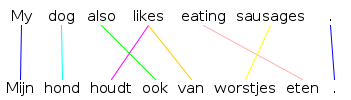
\includegraphics[scale=0.6]{alignment.png}
\caption{A one-to-many alignment of the English sentence `My dog also likes eating sausages.' and its translation `Mijn hond houdt ook van worstjes eten'.%schrijf welke tool is gebruikt
\cite{maillette2010visualizing}
}\label{fig:alignment}
\end{figure}

Alignments can be of several types, which will be of importance for the complexity of our algorithms. A summary can be found in table \ref{table:alignments}.


\begin{table}[!ht]
%Put a box around this thing!!
\begin{tabular}{ll}
one-to-one & $\forall x\forall y \big( (x,y)\!\in\!y \to \forall z \big( (z,y)\!\in\!a \to z\!=\!x \land (x,z) \!\in\! a \to z\!=\!y \big ) \big ) $\\
&\\
one-to many & $\forall x\forall y \big( (x,y)\!\in\!y \to \forall z \big( (z,y)\in a \to z\!=\!x \big) \big) $\\
&\\
many-to-one & $\forall x\forall y \big( (x,y)\!\in\!y \to \forall z \big( (x,z)\!\in\!a \to z\!=\!y \big) \big ) $\\
&\\
many-to-many & - \\
&\\
monotone & $\forall w \forall x\forall y \forall z \big ( \left ( (x,y)\in a \land (w,z)\in a \land x < w \right ) \to y < z \big )$\\
\end{tabular}
\caption{Alignment types, restrictions}
\label{table:alignments}
\end{table}

For the following definitions, we will introduce a change in notation. In our new notation, alignments are represented as a special sort permutation, in which numbers of the original sequence are allowed to appear more than once, or not at all. We will call such a representation a set-permutation. A set-permutation is defined as follows:

\begin{definition}
Given a source sentence $s = s_0 \ldots s_n$, its translation $t = t_0 \ldots t_m$, and an alignment $a$, let $a(i) = \{j | (i,j)\in a\}$ be the set with target positions that is linked to source position $i$. The set-permutation $\pi$ uniquely describing $a$ is defined as the ordered sequence of sets
$\langle a(0), \ldots, a(n) \rangle$
\end{definition}

The set-permutation $\pi = \pi_0, ..., \pi_n$ describing the alignment showed in Figure \ref{fig:alignment} would thus be $\langle {0}, {1}, {3}, {2,4}, {6}, {5}, {7}\rangle$. In the following definitions it is assumed that there are no unaligned target-words (thus for sentence $s_0^n$, $\bigcup_{i=0}^n \pi_i$ constitutes a contiguous sequence of numbers). The definitions can easily be extended to the case where there are unaligned target words, by only numbering the target positions that are aligned (effectively shifting the position numbers to the left whenever an unaligned word is found).

\subsubsection{Translation Units} To define a tree over an alignment, we need to have a notion of allowed sub sequences. For this, we use a definition analogous to the definitions of phrase pair used in the first phrase based models \citep{och2004alignment}. A phrase pair is a pair of source and target spans [i,j] and [x,y], respectively, such that at least one word in [i,j] is aligned to at least one word in [x,y], and no words in [i,j] are aligned to words outside [x,y] and vice versa. The phrases consistent with the alignment are thus phrases whose translation is also a phrase. Translated in terms of a set-permutations $\pi$, we get the following definition for a translation unit:

\begin{definition}
A span [$i,j$] representing contiguous sequence $s_i\ldots s_j$ of a source sentence whose alignment is represented by set-permutation $\pi = \langle\pi_0 ,\ldots ,\pi_n$ is a possible translation unit iff the union $(\pi_i\cup \ldots \cup \pi_j)$ constitutes a contiguous range of integers, and for every integer $x \in (\pi_i\cup \ldots \cup\pi_j)$ holds that  $x \notin (\pi_0\cup \ldots \cup \pi_{j-1} \cup \ldots\cup\pi_{i+1}\cup\ldots\cup \pi_n)$.
\end{definition}

The set of translation units consistent with the alignment in Figure \ref{fig:alignment} is thus: {[0,0], [1,1], [2,3], [4,4], [5,5], [0,1], [2,3], [4,5], [1,3], [0,4], [2,5], [0,5]}. In which [x,y] includes all words from position $x$ to position $y$. Note that the word 'like' is not a translation unit on its own, as it translates into two non-adjacent words in the Dutch target sentence. The number of translation units in an alignment depends on the type of the alignment and is largest in case of a monotone alignment, that does not restrict the set of possible translation units at all. A completely monotone alignment of a sentence of $n$ words has $\frac{n\times n+1}{2}$ translation units. Note that unaligned words can cause exponential growth in the number of translation units.
%Also introduce the term 'discontinuous translation unit' or translation admissable subsequence?
%Say that translation units preserve the structure within

\subsubsection{Alignment Trees} Given the set of translation units, we can define the set of structures according to which the sentence could have been compositionally translated. To define this set of structures, we firstly introduce the notion of a segmentation of a set-permutation.

\begin{definition}
Let $\pi = \langle \pi_0, \ldots,\pi_n\rangle$ be a set-permutation. A segmentation of $\pi$ is a set of indice $B = \{j_0 = 0, j_1, \ldots ,j_m = n\}$ that segments $\pi$ into $m$ adjacent, non-overlapping and contiguous segments such that for all $0\leq i < m$ holds that the subsequence $\pi_{j_i}\ldots\pi_{j_{i+1}}$ is either a translation unit or part of a discontinuous translation unit.%DIT MOET NOG EVEN ANDERS GELOOF IK
\end{definition}

We can now define the set of alignment trees:

\begin{definition}
%Dit moet misschien nog even anders
Given a source sentence $s = s_0 \ldots s_n$ and the set of its translation units $u = \{u_1,\ldots,u_m\}$. An alignment tree is any tree $T$ satisfying the following conditions 4 conditions:\begin{enumerate}
\item $[0,n]$ is the root of the tree
\item For the set $N = \{n | n is a node in T\}$ holds: $N\supset \{[i,i]| 0\leq i\leq n\}$
\item Every node $n\in N$ is in $u\cup \{[i,i]|$ $0\leq i\leq n\} $
\item For every node $[i,j] \in N$ with children $[x_1,y_1]\ldots [x_n,y_n]$ holds: $x_k = y_k+1$ and $\{x_1,\ldots x_n, y_n\}$ is a segmentation of $[i,j]$ %Dit moet ook net iets anders)
\end{enumerate}
\end{definition}

An alignment may have many different possible alignment trees. The number of alignment trees can be exponential in the length of the sentence, if no restriction is placed on the branching factor of the nodes. Every alignment can be assigned at least one structure, that is completely flat. A possible alignment tree for the running example alignment can be found in Figure \ref{fig:alignment_tree} (the words of the sentence are included for clarity reasons).

\begin{figure}
\Tree [.[0,6] [.[0,1] [.[0,0] my ] [.[1,1] dog ] ] [.[2,6] [.[2,4] [.[2,2] also ] [.[3,3] likes ] [.[4,4] eating ] ] [.[5,6] [.[5,5] eating ] [.[6,6] sausage ] ] ] ] ]
\caption{A possible alignment tree for the alignment of Figure \ref{fig:alignment} \label{fig:alignment_tree}}
\end{figure}

\subsubsection{Hierarchical Alignment Trees}

HATs, as defined in \cite{simaan2013hats}, are a subset of all alignment trees, in which all nodes have a minimal branching factor:

\begin{definition}
A HAT is an alignment tree in which the fourth criterion is replaced by the following:
\begin{enumerate}
\item[4.] For every node $[i,j] \in N$ with children $[x_1,y_1]\ldots [x_n,y_n]$ holds: $x_k = y_k+1$ and $\{x_1,\ldots x_n, y_n\}$ is a segmentation $B$ of $[i,j]$ such that for all other segmentations $B'$ of $[i,j]$ holds that $|B'|\geq |B|$ %Dit moet ook net iets anders)
\end{enumerate}
\end{definition}

Furthermore, the nodes of the HATs are decorated with ITG-like operators, that specify how the target-side HAT can be constructed. An example of a HAT can be found in \ref{fig:hat}.

\begin{figure}
\caption{Example HAT, anders}\label{fig:hat}
\end{figure}

%EXPLAIN BETTER WHY WE WANT THE MAXIMAL BRANCHING FACTOR
With the node labels, a HAT uniquely determines a word-alignment, in a maximally recursive fashion. The latter is desirable, because it maximises the probability that we can generalise to new data. \cite{simaan2013hats} provide empirical data, some of which was discussed in the previous section, describing what percentage of alignments can be explained by constrained versions of HATs. Note that \textit{every} word alignment can be represented by a HAT, if no constraints are imposed.

\subsubsection{The Mapping between HATs}

As mentioned before, the nodes of a HAT are decorated with operators

Until now we have focussed on constructing monolingual structures for the source side of the translation data, without paying much attention to the structure of its translation. The operators on the nodes 
Explain that a tree for the other side can be constructed (node decorations itgs like)
trees need not be isomorphic, mapping between the structures is not bijective (but if the reorder operators are seen as labels they are)

Maybe give some examples? Tell what kind of mapping it describes
Explain that it mostly means that the trees don't have to be isomorphic
bijective mapping to structures

\subsection{The Power of HATs}

Besides the phenomena covered by SCFG's, HATs can account for a 
%Explain the power of HATs, give some examples

\subsection{Experiments}

Before describing our experiment, recall that the main aim of this paper is investigating the assumptions underpinning compositional translation. In particular, we want to see if it is possible to find recursive structures of sentences and a systematic mapping between them. The HATs are a very powerful tool for doing so, as they can describe any translation from source to target side. However, the mapping from word-alignments to HATs is a one-to-many mapping: a HAT uniquely describes a word-alignment, but a word alignment is often described by many HATs. To confirm that compositional translation is a reasonable strategy, we need somewhat stronger: a way of producing a single HAT for a word alignment, that is consistent over all sentences.\footnote{There are two remarks needed to refine this statement. Firstly we assume that a sentence has only one meaning, ambiguity cases are thus ruled out. If a sentence has multiple meanings, different HATs might correspond to these meanings. This thesis considers such ambiguity aspects a separate problem, which (that?) is not taken into account here at all. Secondly, it is mainly theoretical that we want to fine \textit{one} HAT per alignment. This is not to say, that in practice is might not be more desirable to generate multiple HATs per sentence over which a probability distribution can be defined. (anders)} In this thesis we are concerned with finding such a consistent set of HATs for a corpus. There can be exponentially many HATs per sentence (compute how many), and statistical learning this set without any external reference seems out of reach. Given that the nature of translation is preservation of the semantic content of a sentence, it seems reasonable to assume that the structural representation of a translation is semantically motivated. As guide in our search we will therefore use dependency parses \cite{schubert1987metataxis}, that specify the predicate argument structure of a sentence as perceived by humans, hereby implicitly addressing the question: are predicate argument structures preserved during translation. As many proceeding empirical investigations, we will only focus on source side structures (at first), not worrying about the consistency of the target side structures they are mapped to, implying that we will not consider the node operators. If no consistent source side structures can be found, there is no hope for finding consistent pairs of structures.

\subsubsection{Experiment 1}

The predicate argument relations in a dependency tree, tell us exactly how the sentence is composed: we can infer which are the smaller parts of the sentence and how they are combined to obtain the complete sentence. Consider for instance the dependency tree of the sentence "My dog also likes eating sausage" (Figure \ref{fig:deptree1}).

\begin{figure}[!h]\label{fig:deptree1}
\centering
\begin{dependency}[theme=simple]%[hide label]
\begin{deptext}[column sep=.5cm, row sep=.1ex]
%PRP\$ \& NN \& RB \&[.5cm] VBZ \& VBG \& NN \\
My \& dog \& also \& likes \& eating \& sausage \\
\end{deptext}
\deproot{4}{}
\depedge{2}{1}{poss}
\depedge{4}{2}{nsubj}
\depedge{4}{3}{xvmod}
\depedge{4}{5}{xcomp}
\depedge{5}{6}{dobj}
\end{dependency}
\caption{Stanford Dependency Tree}
\end{figure}

The dependency tree tells us that 'likes' is the head word of the sentence, and that the sentences is composed of 4 parts: the head 'likes', its modifier 'also', its noun subject whose head is 'dog' and the open clausal complement whose head is 'eating'. The complement and subject are further divisible in, 'My' and 'dog', and 'eating' and 'sausage', respectively. Intuitively, for every relation in the dependency parse, we can check whether this relation exists in a HAT by checking if the word and its depending subtrees are siblings in the HAT.
In a first experiment, for every alignment, we will search for the HAT in which the number of dependency relations that is consistent with the HAT is the highest. We will assign a score to the HAT, proportional to the percentage of dependencies that is respected. A formal definition of this metric can be found in \ref{appendix:metric}.
%Maybe something about how phrasal translations come into play

\subsubsection{Follow-up Experiments}

In the best case, we can find a HAT for every sentence in which all dependency relations are preserved, but we suspect that this will not be so, in which cae we will further investigate if the result can be improved. We have distinguished five reasons that could lead to a low score:

\begin{enumerate}
\item The translation is erroneous, or non literal;
\item The dependency parse is erroneous;
\item The alignment is erroneous;
\item The structure of HATs and dependency parses does not agree
\item The sentence cannot be compositionally translated.
\end{enumerate}

Research like this hinges on the assumption that the datasets we use are representative for the phenomena we are investigating, and don't contain to many mistakes (anders). Unfortunately, this is often not the case. Dependency parsers are not perfect, the translations in our corpora are often not as literal as we would want them to be, and automatic alignments often contain many incorrect alignment links. Although these factors can play an important role, there is not much that we can do about it: we cannot instruct interpreters of the government to follow a protocol we like, and we do not have the manpower to filter our corpora or produce manual alignments for corpora of a reasonable size. Even in empirical research, testing the influence of these factors often boils down to manually checking the data. We will consider the influence of the alignments, by running the same experiments on manually aligned datasets. As regards the first two causes, we might perform a manual analysis on a small subset of our data, but not before we have investigated the fourth case, which we consider likely to be an issue as we have forced our trees to be maximally recursive. This is very useful for computational purposes, but is likely not the structure corresponding to human intuitions. We will illustrate this with two examples.\\
Firstly, consider the sentence `I give you flowers', which contains one predicate ('give') with three arguments (the subject `I', the object `flowers' and the indirect object `you'). Its Dutch translation `Ik geef jou bloemen' has exactly the same predicate argument structure \textit{and} word-order, whereby the branching factor in any of its HATs will not exceed 2. However, a maximum score can only be obtained by a tree in which `I', `give', `you', and `flowers' are siblings, whose mother will have a branching factor of (at least) 4. Even though the translation of this sentence seems perfectly compositional, no HAT will thus obtain the maximum score, because the dependency structure is not minimally branching.\\
A second example, that is more related to translational divergence, arises when two arguments are translated into one (which happens when e.g. arguments are translated are pre or suffixes, verbs do not require a subject or when spaces). Consider for instance the sentence 'Can you give me the salt' and its Italian translation 'puoi passarmi il sale'. Once again, this translation seems compositional. However, the dependency parse prescribes that `the salt', `can' and `you' should be siblings of `give', which will be the case in none of the HATs over $\{\{0\},\{0\},\{1\},\{1\},\{2\},\{3\}\}$, as `give' and `me' are together translated into `passarmi', and `can you' into `puoi'.\\
%Anders
Both cases could be solved when considering dependency motivated labels, similar to the ones defined in \cite{zollmann2006syntax}, that represent compound categories, which we will do in a second experiment. E.g. `give you flowers' could be seen as a sentence missing a subject to the left (subj\textbackslash S) and `I give' as a combination of a subject and a verb (subj+verb). We will investigate this new labels by obtaining some statistical details about how often they are respected by the alignments. Subsequently, we will rescore the HATs with the new labels, slightly adapting the scoring metric. Instead for looking at sibling relations, we will just consider how many of the nodes in the HAT can be labelled using a label from our new label set. A HAT will receive a score corresponding with the percentage its nodes that could be labelled and thus receives a maximum score if all of its nodes could be labelled. Note that this introduces a slight bias towards trees with more nodes: a tree with 10 nodes of which one is unlabelled receives a higher score than a tree with 9 nodes of which one is unlabelled. %Explain why we do not think this is problematic?




%%%%%%%%%%%%%%%%%%%%%%%%%%%%%%%%%%%%%%%%%%%%%%%%%%%%%%%%%%%%%%%%%%%%%%%%%%%%%%%%%%%%%%%%%%%%%%%%%%%%%%%%%%%%%%%%%%%%%%%%%%%%%%%%%%%%%%%%%%%%%%%%%%%%%%
%%%%%%%%%%%%%%%%%%%%%%%%%%%%%%%%%%%%%%%%%%%%%%%%%%%%%%%%%%%%%%%%%%%%%%%%%%%%%%%%%%%%%%%%%%%%%%%%%%%%%%%%%%%%%%%%%%%%%%%%%%%%%%%%%%%%%%%%%%%%%%%%%%%%%%
% EXPERIMENTS
%
% Describing the experiments and their results
%


\chapter{Results}

This chapter will describe the sequence of experiments we conducted, as well as their results. Implementation details can be found in \ref{appendix:impl}. 




% What I want to describe now: ran test experiments on a small dataset, results: HATs do not capture compositionality as in the dependency parses, a small problem are the alignments, but a bigger problem is that the structure from the compositionality derived from the dependency parses is not minimally branching (test with ALL trees)
% but our goal is to find a consistent set of structures (i.e. consistently label them), so maybe we can do it diffently
% Investigate which relations ARE preserved, investigation on bigger dataset, find which relations are preserved and which aren't and see which ones are preserved an which ones aren't, maybe we can now investigate new labels?




% END OF RESULTS
%%%%%%%%%%%%%%%%%%%%%%%%%%%%%%%%%%%%%%%%%%%%%%%%%%%%%%%%%%%%%%%%%%%%%%%%%%%%%%%%%%%%%%%%%%%%%%%%%%%%%%%%%%%%%%%%%%%%%%%%%%%%%%%%%%%%%%%%%%%%%%%%%%%%%%
%%%%%%%%%%%%%%%%%%%%%%%%%%%%%%%%%%%%%%%%%%%%%%%%%%%%%%%%%%%%%%%%%%%%%%%%%%%%%%%%%%%%%%%%%%%%%%%%%%%%%%%%%%%%%%%%%%%%%%%%%%%%%%%%%%%%%%%%%%%%%%%%%%%%%%





%%%%%%%%%%%%%%%%%%%%%%%%%%%%%%%%%%%%%%%%%%%%%%%%%%%%%%%%%%%%%%%%%%%%%%%%%%%%%%%%%%%%%%%%%%%%%%%%%%%%%%%%%%%%%%%%%%%%%%%%%%%%%%%%%%%%%%%%%%%%%%%%%%%%%%
%%%%%%%%%%%%%%%%%%%%%%%%%%%%%%%%%%%%%%%%%%%%%%%%%%%%%%%%%%%%%%%%%%%%%%%%%%%%%%%%%%%%%%%%%%%%%%%%%%%%%%%%%%%%%%%%%%%%%%%%%%%%%%%%%%%%%%%%%%%%%%%%%%%%%%
% DISCUSSION
%
%

\chapter{Discussion and Future Work}

short summary of findings and what they mean

%future work: source reordering, treebank to learn translation structure
% promising for further models: monolingual parsing and learning reordering operators


%
% 
% END OF DISCUSSION
%%%%%%%%%%%%%%%%%%%%%%%%%%%%%%%%%%%%%%%%%%%%%%%%%%%%%%%%%%%%%%%%%%%%%%%%%%%%%%%%%%%%%%%%%%%%%%%%%%%%%%%%%%%%%%%%%%%%%%%%%%%%%%%%%%%%%%%%%%%%%%%%%%%%%%
%%%%%%%%%%%%%%%%%%%%%%%%%%%%%%%%%%%%%%%%%%%%%%%%%%%%%%%%%%%%%%%%%%%%%%%%%%%%%%%%%%%%%%%%%%%%%%%%%%%%%%%%%%%%%%%%%%%%%%%%%%%%%%%%%%%%%%%%%%%%%%%%%%%%%%




%%%%%%%%%%%%%%%%%%%%%%%%%%%%%%%%%%%%%%%%%%%%%%%%%%%%%%%%%%%%%%%%%%%%%%%%%%%%%%%%%%%%%%%%%%%%%%%%%%%%%%%%%%%%%%%%%%%%%%%%%%%%%%%%%%%%%%%%%%%%%%%%%%%%%%
%%%%%%%%%%%%%%%%%%%%%%%%%%%%%%%%%%%%%%%%%%%%%%%%%%%%%%%%%%%%%%%%%%%%%%%%%%%%%%%%%%%%%%%%%%%%%%%%%%%%%%%%%%%%%%%%%%%%%%%%%%%%%%%%%%%%%%%%%%%%%%%%%%%%%%
% CONCLUSION
%
%

\chapter{Conclusion}

%
%
% END OF CONCLUSION
%%%%%%%%%%%%%%%%%%%%%%%%%%%%%%%%%%%%%%%%%%%%%%%%%%%%%%%%%%%%%%%%%%%%%%%%%%%%%%%%%%%%%%%%%%%%%%%%%%%%%%%%%%%%%%%%%%%%%%%%%%%%%%%%%%%%%%%%%%%%%%%%%%%%%%
%%%%%%%%%%%%%%%%%%%%%%%%%%%%%%%%%%%%%%%%%%%%%%%%%%%%%%%%%%%%%%%%%%%%%%%%%%%%%%%%%%%%%%%%%%%%%%%%%%%%%%%%%%%%%%%%%%%%%%%%%%%%%%%%%%%%%%%%%%%%%%%%%%%%%%



%%%%%%%%%%%%%%%%%%%%%%%%%%%%%%%%%%%%%%%%%%%%%%%%%%%%%%%%%%%%%%%%%%%%%%%%%%%%%%%%%%%%%%%%%%%%%%%%%%%%%%%%%%%%%%%%%%%%%%%%%%%%%%%%%%%%%%%%%%%%%%%%%%%%%%
%%%%%%%%%%%%%%%%%%%%%%%%%%%%%%%%%%%%%%%%%%%%%%%%%%%%%%%%%%%%%%%%%%%%%%%%%%%%%%%%%%%%%%%%%%%%%%%%%%%%%%%%%%%%%%%%%%%%%%%%%%%%%%%%%%%%%%%%%%%%%%%%%%%%%%
% APPENDIX IMPLEMENTATION
%
%

\appendix
\chapter{Implementation}
\label{appendix:impl}

NLTK toolkit: \cite{bird2009natural}\\
Stanford Dependency Parser: \cite{de2008stanford}(?)

%
%
% END OF APPENDIX IMPLEMENTATION
%%%%%%%%%%%%%%%%%%%%%%%%%%%%%%%%%%%%%%%%%%%%%%%%%%%%%%%%%%%%%%%%%%%%%%%%%%%%%%%%%%%%%%%%%%%%%%%%%%%%%%%%%%%%%%%%%%%%%%%%%%%%%%%%%%%%%%%%%%%%%%%%%%%%%%
%%%%%%%%%%%%%%%%%%%%%%%%%%%%%%%%%%%%%%%%%%%%%%%%%%%%%%%%%%%%%%%%%%%%%%%%%%%%%%%%%%%%%%%%%%%%%%%%%%%%%%%%%%%%%%%%%%%%%%%%%%%%%%%%%%%%%%%%%%%%%%%%%%%%%%



%%%%%%%%%%%%%%%%%%%%%%%%%%%%%%%%%%%%%%%%%%%%%%%%%%%%%%%%%%%%%%%%%%%%%%%%%%%%%%%%%%%%%%%%%%%%%%%%%%%%%%%%%%%%%%%%%%%%%%%%%%%%%%%%%%%%%%%%%%%%%%%%%%%%%%
%%%%%%%%%%%%%%%%%%%%%%%%%%%%%%%%%%%%%%%%%%%%%%%%%%%%%%%%%%%%%%%%%%%%%%%%%%%%%%%%%%%%%%%%%%%%%%%%%%%%%%%%%%%%%%%%%%%%%%%%%%%%%%%%%%%%%%%%%%%%%%%%%%%%%%
% APPENDIX EVALUATION METRICS
%
%

\chapter{Metrics}
\label{appendix:metric}

\section{Notation}

Firstly, we will present some notation that is shared along the different metrics.

\begin{notion}
$T_d$ will refer to a dependency tree of a sentence $s = w_1 \dots w_n$, formed by a set of dependencies $D = \{ (i,j) |$ there is a dependency arrow from word $w_i$ to word $w_j \}$.
\end{notion}

\begin{notion}
If $T_d$ is a dependency tree for $s$, $w$ is a word in $s$ and $i$ and $j$ are the maximum and minimum positions, respectively, that can be reached from $w$ by following the directed dependency arrows. Then span($w$) = $[i,j]$.
\end{notion}

\begin{notion}
$T_a$ will be used to refer to an alignment tree of a sentence $s = w_1 \dots w_n$. The label $i-j$ will refer to the node that dominates span $[i,j]$. The highest node of $T_a$ will be denoted with $N_{T_a}$
\end{notion}

\begin{notion}
Let $T_d$ be a dependency tree with dependencies $D$, Then $D' = \{ (i,\textrm{span}(j))$ $|$ $D(i,j) \land 1 \leq i,j \leq n \}$ is the set in which each dependent is replaced by its span.
\end{notion}

\begin{notion}
If $N$ is a node in a tree $T_a$, $C_N$ denotes the set of child constituents of this node. If node $N$ dominates words $i$ to $j$ in $s$, then $dom(N)= [i,j]$
\end{notion}

\section{Metric 1}

\begin{metric}\label{m1}
Let $s = w_1 w_2 \dots w_n$ be a sentence, and $T_d$ and $T_a$ its dependency tree and an alignment tree, respectively. The score of $T_a$ is defined as the score of its highest node $N_{a}$:

$$
E(N_a,D) = \sum_{c\in C_{N_a}} E(c,D)+ \sum_{c_1\in C_{N_a}} \sum_{c_2\in C_{N_a}} B(c_1,c_2)
$$

\noindent With base case $E(N,D) = 0$ and $B(c_1,c_2) = 1$ iff  $(c_1,c_2)\in D'$. Dividing the resulting score by $|D'|$ will result in a normalized score.
\end{metric}

\noindent  Note if this definition is strictly followed more than half of the sibling checks is redundant, an algorithm computing the score of a tree would not have to perform them all.

\section{Metric 2}

\begin{metric}\label{m2}
Let $s = w_1 w_2 \dots w_n$ be a sentence, and $T_d$ and $T_a$ its dependency tree and an alignment tree, respectively. The score of $T_a$ is defined as the score of its highest node $N_{a}$:

$$
E(N_a,D) = \sum_{c\in C_{N_a}} E(c,D)+ \sum_{c_1\in C_{N_a}} \sum_{c_2\in C_{N_a}} B(c_1,c_2)
$$

\noindent With base case $E(N,D) = 0$ and $B(c_1,c_2) = 1$ iff  $|dom(c_2)| > 1 \land (c_1,c_2)\in D'$ the part of the sentence covered by $c_2$. Dividing the resulting score by $|D'|$ will result in a normalized score.
\end{metric}

Note that normalizing the score will sometimes result in zero division for shorter sentences whose dependency parses display no compositional structure, in this cases we will define the score of the sentence to be 0.


\subsection{Metric 1}


\subsection{Metric 2}

Explain that metric 1 reflects the similarity with the dependency parse, rather than giving a reasonable measure of compositionality. Explain why this is, that a part of the score can trivially be reached by just making a flat tree. Explain how to fix this. Explain that evaluation metric 2 won't alter the ordering of the trees, just their scores.
Explain that metric 2 thus just differs in the set of relations it considers: instead of considering all relations from the dependency parse, it only considers the relations that reflect compositionality, which captures the intuition that completely flat trees should be assigned a 0 score. Note that this means that this therefore does not alter the ranking of the trees set by metric 1, it just alters the scores associated with the trees.








%%%%%%%%%%%%%%%%%%%%%%%%%%%%%%%%%%%%%%%%%%%%%%%%%%%%%%%%%%%%%%%%%%%%%%%%%%%%%%%%%%%%%%%%%%%%%%%%%%%%%%%%%%%%%%%%%%%%%%%%%%%%%%%%%%%%%%%%%%%%%%%%%%%%%%
%%%%%%%%%%%%%%%%%%%%%%%%%%%%%%%%%%%%%%%%%%%%%%%%%%%%%%%%%%%%%%%%%%%%%%%%%%%%%%%%%%%%%%%%%%%%%%%%%%%%%%%%%%%%%%%%%%%%%%%%%%%%%%%%%%%%%%%%%%%%%%%%%%%%%%

%THINGS I SHOULDN'T FORGET TO MENTION!

% zeg iets over dat we op deze manier nicely omgaan met phrasal translations

% put statistics about the data, the dependency parses, everything

% ook wat analyses over complexiteit e.d. max grootte van de grammatica's dat soort zaken

% niet zo tevreden over hoe dependency grammars met conjunction omgaan, collapsed dependencies doen dit wel beter trouwens, misschien moet ik daar nog eens naar kijken. Collapsed dependencies doen soms ook al wat werk met idiom (zie tabel 3)

%Geen enkel vertaalsysteem vertaalt een zin 'in zijn geheel', altijd in stukken

% Bouw iets in in dat dependency programma dat oneindige recursie tegengaat

% Bouw meer checks in die kijken of de input wel consistent is

% Zeg ergens iets over dat vertalers ook vaak de keuze maken om iets niet letterlijk te vertalen, maar dat we er hier vanuit gaan dat dit wel gebeurt (of iig zo letterlijk mogelijk)

% A compositional approach ideally takes care of several problems at the same time

% Ergens moet ik ook nog de vraag stellen of we de semantiek en de syntax echt apart nodig hebben (zoals in Rosetta). 

\bibliography{thesisDH}

\end{document}
